\section{Toy Examples}

Figure~\ref{fig:toy-regret} summarizes the expanded toy family. In the
packing-style examples, two-stage prediction changes the selected solution but
the normalized gap remains below the 5\% reference line. In the path-like
controls, a ranking error redirects the whole connected path and creates much
larger regret.

\begin{figure}[t]
    \centering
    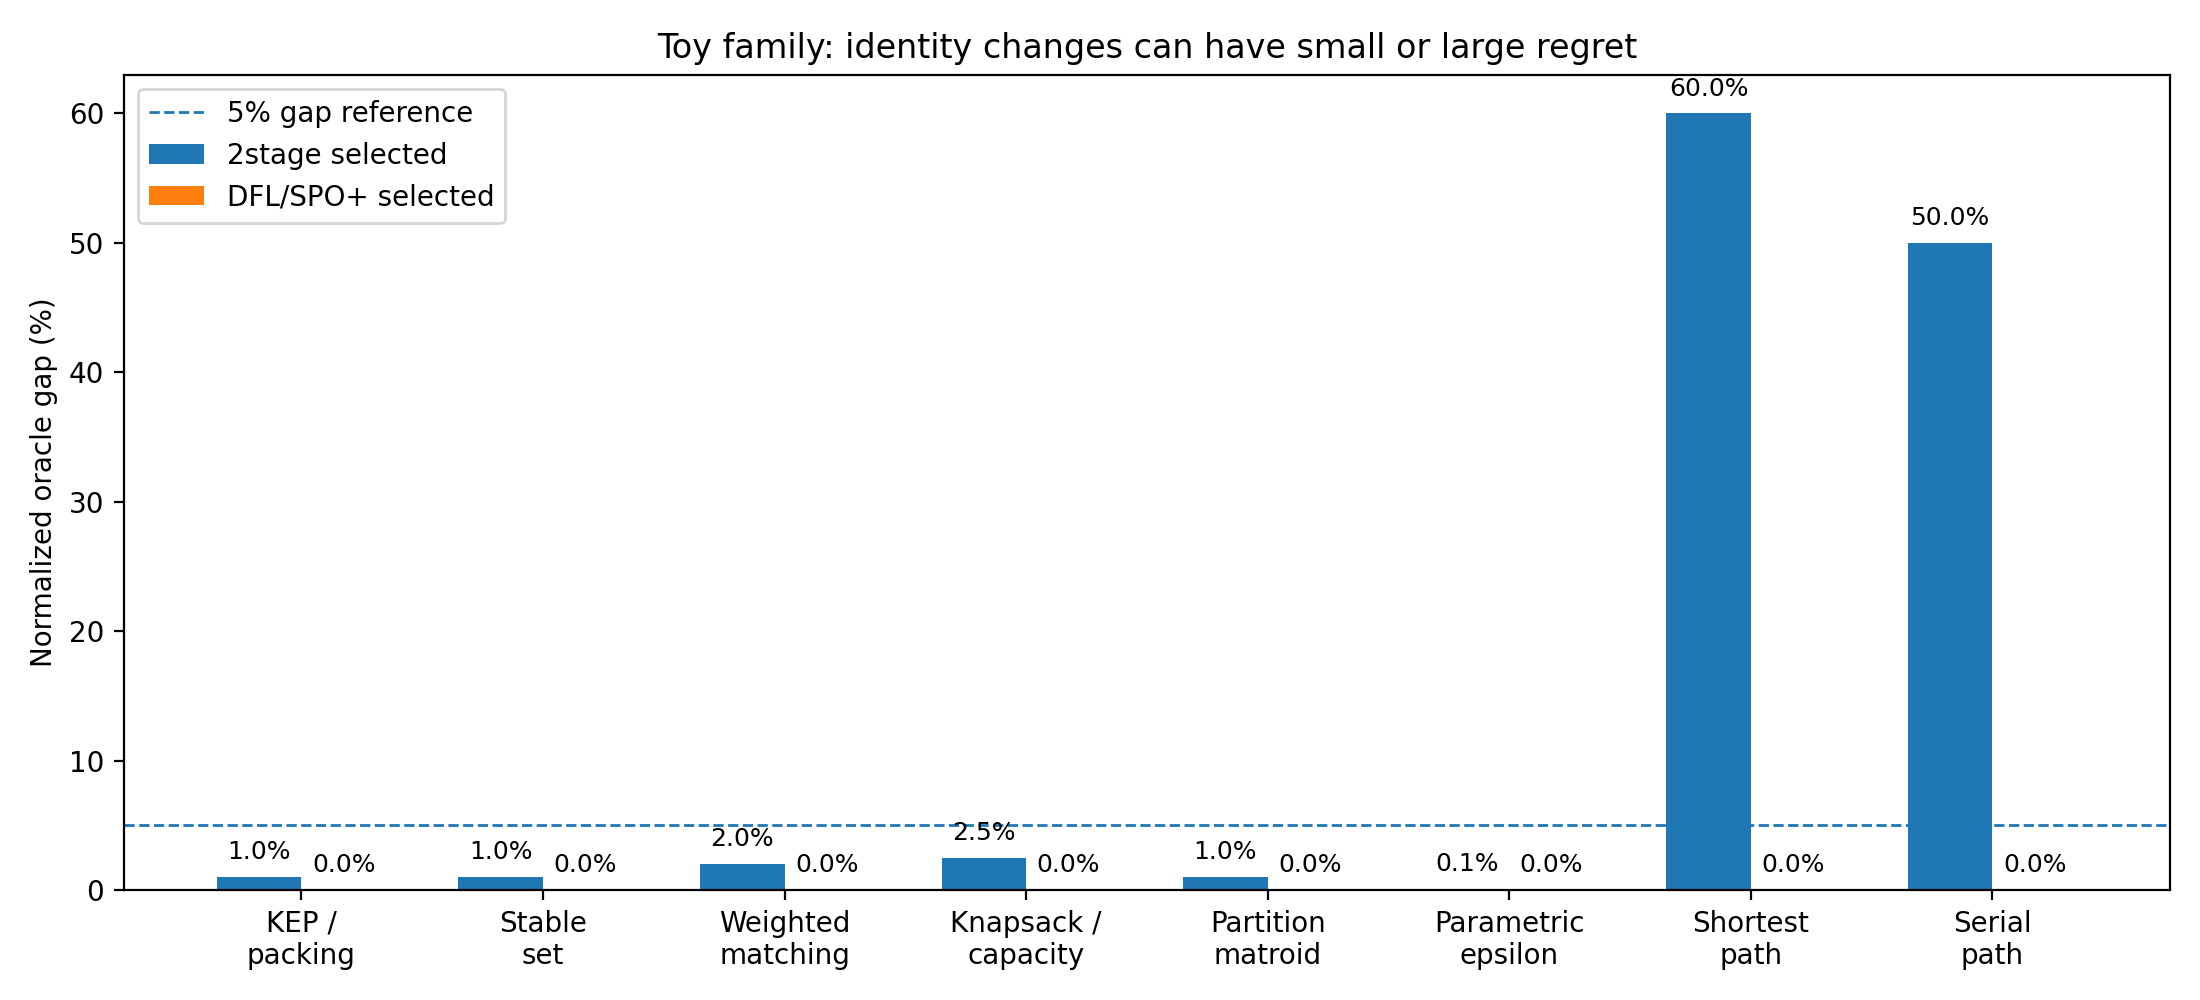
\includegraphics[width=\linewidth]{figures/toy_regret_comparison.png}
    \caption{Toy family showing that solution identity changes can correspond
    to either small or large regret. Packing-style positive examples have close
    substitutes; path-like negative controls do not.}
    \label{fig:toy-regret}
\end{figure}

\begin{figure}[t]
    \centering
    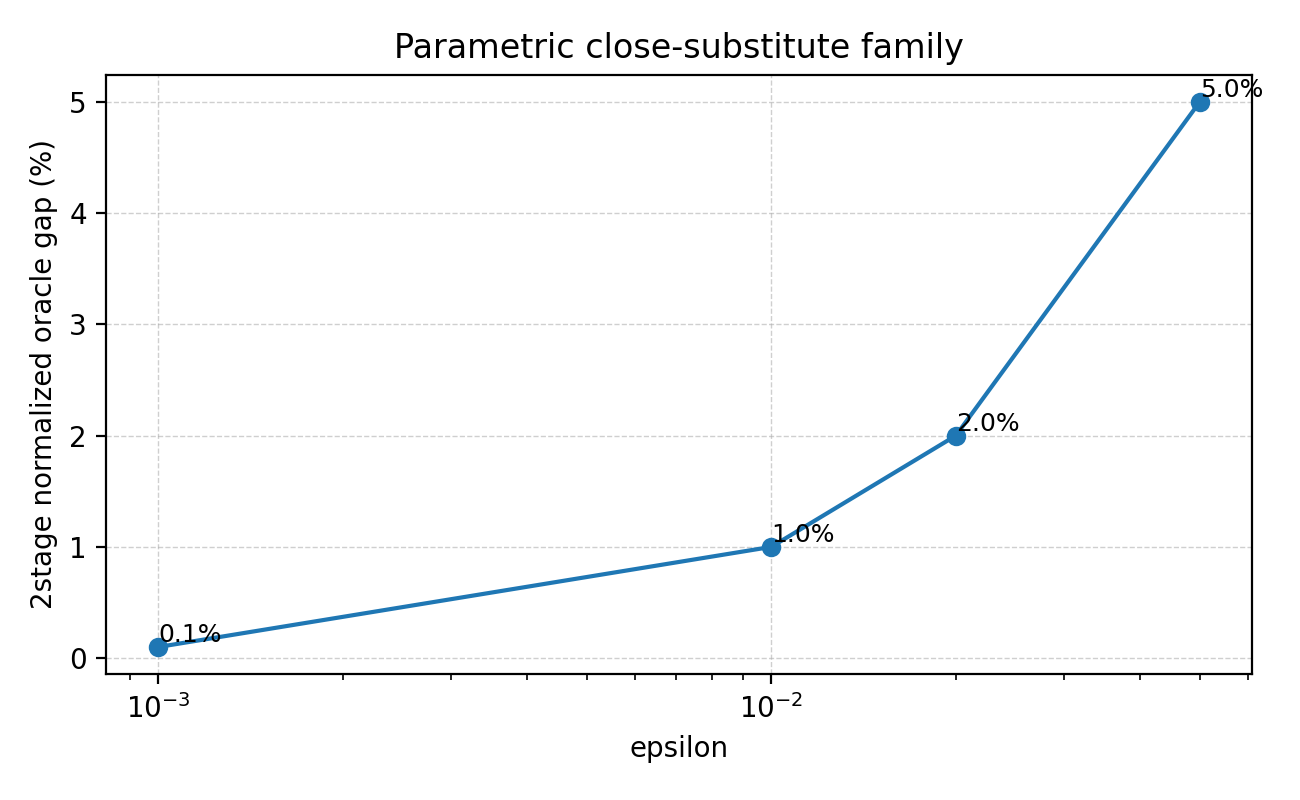
\includegraphics[width=\linewidth]{figures/toy_parametric_epsilon_curve.png}
    \caption{Parametric close-substitute construction. The selected solution
    changes for every $\epsilon$, but the normalized regret is exactly
    $\epsilon$ and can be made arbitrarily small.}
    \label{fig:toy-epsilon}
\end{figure}

Table~\ref{tab:toy-summary} lists the oracle and two-stage selected solutions
for each toy problem family.

\begin{table*}[t]
    \centering
    \caption{Toy examples for the close-substitute mechanism and path-like
    negative controls.}
    \label{tab:toy-summary}
    \small
    \setlength{\tabcolsep}{3pt}
    \begin{tabular}{llll}
\toprule
Problem & Oracle / true best & 2stage selected & 2stage normalized gap \\
\midrule
KEP / set packing & C12 + C34, value 20 & C13 + C24, value 19.8 & 1.0\% \\
Stable set & A + B, value 20 & C + D, value 19.8 & 1.0\% \\
Weighted matching & M12 + M34, value 20 & M13 + M24, value 19.6 & 2.0\% \\
Cardinality knapsack & A + B, value 20 & C + D, value 19.5 & 2.5\% \\
Partition matroid & A1 + B1, value 20 & A2 + B2, value 19.8 & 1.0\% \\
Parametric packing family & S\_star, value 1 & S\_epsilon, value 0.999 & 0.1\% \\
Shortest path & Path A: s-a1-a2-t, cost 5 & Path B: s-b1-b2-t, cost 8 & 60.0\% \\
Serial path control & Serial route A: low-cost chain, cost 10 & Serial route B: high-cost chain, cost 15 & 50.0\% \\
\bottomrule
\end{tabular}

\end{table*}

The parametric construction is the most direct generality argument. It contains
two complete feasible solutions, $S_\star$ and $S_\epsilon$, with true values
$1$ and $1-\epsilon$. If the two-stage predictor slightly overestimates
$S_\epsilon$, it selects the wrong solution identity. Nevertheless, normalized
regret is only $\epsilon$.
